\iffalse
\let\negmedspace\undefined
\let\negthickspace\undefined
\documentclass[journal,12pt,twocolumn]{IEEEtran}
\usepackage{cite}
\usepackage{amsmath,amssymb,amsfonts,amsthm}
\usepackage{algorithmic}
\usepackage{graphicx}
\usepackage{textcomp}
\usepackage{xcolor}
\usepackage{txfonts}
\usepackage{listings}
\usepackage{enumitem}
\usepackage{mathtools}
\usepackage{gensymb}
\usepackage{comment}
\usepackage[breaklinks=true]{hyperref}
\usepackage{tkz-euclide} 
\usepackage{listings}
\usepackage{gvv}  
\usepackage{circuitikz}
\usetikzlibrary{intersections}
\usepackage{tikz}
\def\inputGnumericTable{}                                 
\usepackage[latin1]{inputenc}                                
\usepackage{color}                                            
\usepackage{array}                                            
\usepackage{longtable}                                       
\usepackage{calc}                                             
\usepackage{multirow}                                         
\usepackage{hhline}                                           
\usepackage{ifthen}                                           
\usepackage{lscape}


\newtheorem{theorem}{Theorem}[section]
\newtheorem{problem}{Problem}
\newtheorem{proposition}{Proposition}[section]
\newtheorem{lemma}{Lemma}[section]
\newtheorem{corollary}[theorem]{Corollary}
\newtheorem{example}{Example}[section]
\newtheorem{definition}[problem]{Definition}
\newcommand{\BEQA}{\begin{eqnarray}}
\newcommand{\EEQA}{\end{eqnarray}}
\newcommand{\define}{\stackrel{\triangle}{=}}
\theoremstyle{remark}
\newtheorem{rem}{Remark}

\begin{document}
\bibliographystyle{IEEEtran}
\vspace{3cm}
\title{\textbf{IN-2023}}
\author{EE23BTECH11053-R.Rahul$^{*}$% <-this % stops a space
}
\maketitle
\newpage
\bigskip

\textbf{QUESTION:}\\
61. In the diagram shown, the frequency of the sinusoidal source voltage $V_s$ is 50 Hz.The load voltage is 230 V (RMS), and the load impedance is $\frac{230}{\sqrt{2}}$+$j\frac{230}{\sqrt{2}}$ $\Omega$. The value of attenuator $A_1$=$\frac{1}{50\sqrt{2}}$.The multiplier output voltage $V_o=\frac{V_xV_y}{1V}$, where $V_x$ and $V_y$ are the inputs. The magnitude of the average value of the multiplier output $V_0$ is \hspace{3cm}\rule{5cm}{0.4pt} V

\vspace{1cm}

\begin{circuitikz}
    \draw (0,0) to[sV, l=$V_s$] (0,3) -- (6,3) ;
    \draw [european](6,3) to[R, l=Load ](6,0)  --(2,0)  ;
     \draw (5.4,0) to  (5.1,0);
    \draw (2,0) to[R, l=$1 \Omega$]   (0,0);
    \draw (5.25,3) to (5.25,-4.75) -- (4.25,-4.75) ;
    \draw  (4.25,-4) rectangle (3.25,-5) node [midway] {$A_1$};
    \draw (0,0) node[ground]{};
    \draw (4.75,0) to (4.75,-4.35) -- (4.25,-4.35);
   \draw (3.25,-4.5) to (3,-4.5);
    \draw (3,-4) rectangle(-0.5, -5) node [midway] {$+90^\circ$ phase  
    shifter};
    \draw (2.5,-4) to (2.5,-3.5) -- (3, -3.5)-- (3,-2.5) -- (2.5, -1.6339746) --(2,-2.5) -- (2,-3.5) -- (2.5,-3.5); 
    \node at (2.25,-3.75) {$V_y$};
    \draw (2, -2.5) to (3, -3.5);
    \draw (3,-2.5) to (2,-3.5) ;
    \draw (4,0) to (4,-3.25) -- (3,-3.25);
     \node at (3.25,-3) {$V_x$};
    \draw (2.5, -1.3)   to   (2.5, -1.6339746) ;
    \node at (2.15,-1.3) {$V_o$};
\end{circuitikz}

\vspace{2cm}		
	
\solution
\fi
\begin{table}[h]
  \centering
  \renewcommand{\arraystretch}{1.5}
\begin{tabular}{|c|c|c|}
\hline
Parameter & Description & Value \\\hline
\( V_s \) & sinusoidal Source voltage & 230 V(RMS)\\ \hline
\(V_1 \) & voltage across attenuator &  \\\hline
\( V_x and V_y \) & inputs voltages& \\ \hline
\(A_1\) & attenuator&  $\frac{1}{50\sqrt{2}}$ \\ \hline
\(Z\) & Load Impedance& $\frac{230}{\sqrt{2}}+j\frac{230}{\sqrt{2}}$ $\Omega$ \\ \hline
\(V_0\) & output voltage & $V_0=\frac{V_xV_y}{1V} $\\ \hline
\end{tabular}
\caption{variables}
  \label{tab:xn}
\end{table}
\begin{enumerate}
    \item 

Let the curret in load be I

\begin{center}
\begin{align}
     I &=\frac{V_s(peak)}{Z}\\
     &=\frac{230\sqrt{2}}{\frac{230}{\sqrt{2}}+j\frac{230}{\sqrt{2}}} \\
     &=\sqrt{2}(1-j)
\end{align}
\end{center}
\item
voltage at attenuator 
\begin{align}
    V_1&=V_sA_1\\
    &=230\frac{1}{50\sqrt{2}}V\\
    &=\frac{4.6}{\sqrt{2}}V
\end{align}

\begin{center}
    \begin{align}
        V_y&=4.6\sin(\omega t+90^\circ)\\
        V_x&=I\times 1\Omega\\
        &=2\sqrt{2}\sin(\omega t-45^\circ)\\
        V_0&=9.2\sqrt{2}(\frac{\cos(135)-\cos(2\omega t)}{2})\\
        &=4.6-4.6\sqrt{2}\cos(2\omega t)\\
    \end{align}
\end{center}

\item 
Let f(t)= $4.6-4.6\sqrt{2}\cos(2\omega t)$
\begin{align}
    V_o<avg>&=\frac{1}{T}\int_{0}^{T}(4.6-4.6\sqrt{2}\cos(2\omega t))\,dt\\
    &=\frac{\omega}{\pi} \left[\int_{0}^{\frac{\pi}{\omega}}4.6\,dt-4.6\sqrt{2}\int_{0}^{\frac{\pi}{\omega}}\cos(2\omega t)\,dt\right]\\
    &=\frac{\omega}{\pi}\left[4.6\frac{\pi}{\omega}-4.6\sqrt{2}\left[\frac{\sin(2\pi )}{2\omega}\right]\right]\\
    &=4.6
\end{align}
\end{enumerate}
\begin{figure}[h]
      \centering
       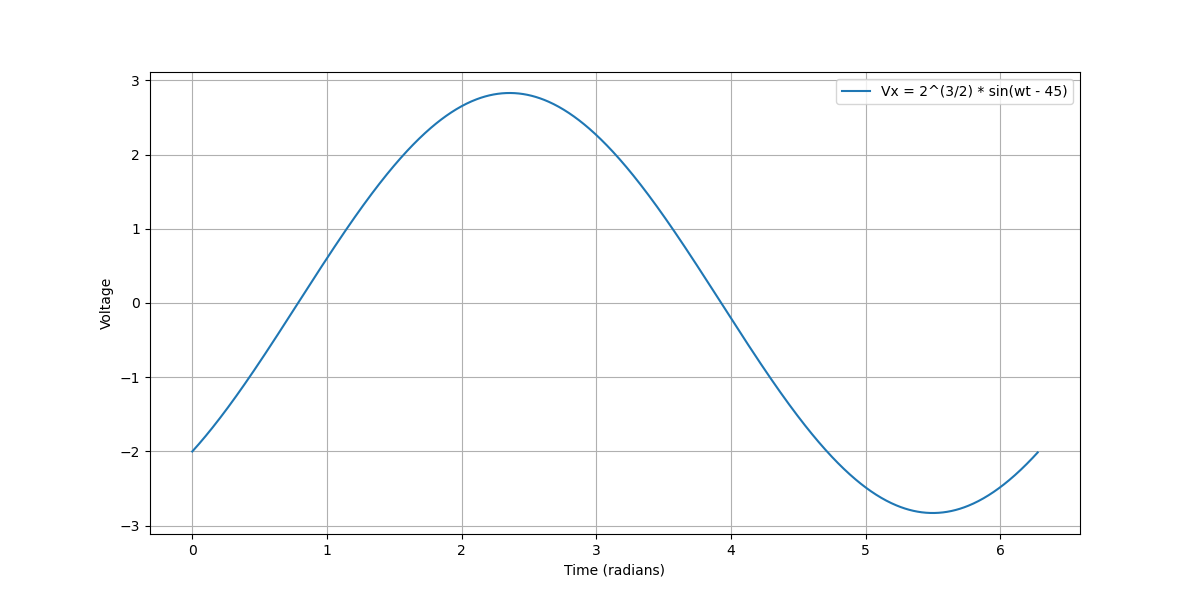
\includegraphics[width=1\linewidth]{2023/IN/61/figs/V_x.png} % Adjust the width as needed
        \caption{$plot of V_x$}
\end{figure}
\begin{figure}[h]
      \centering
       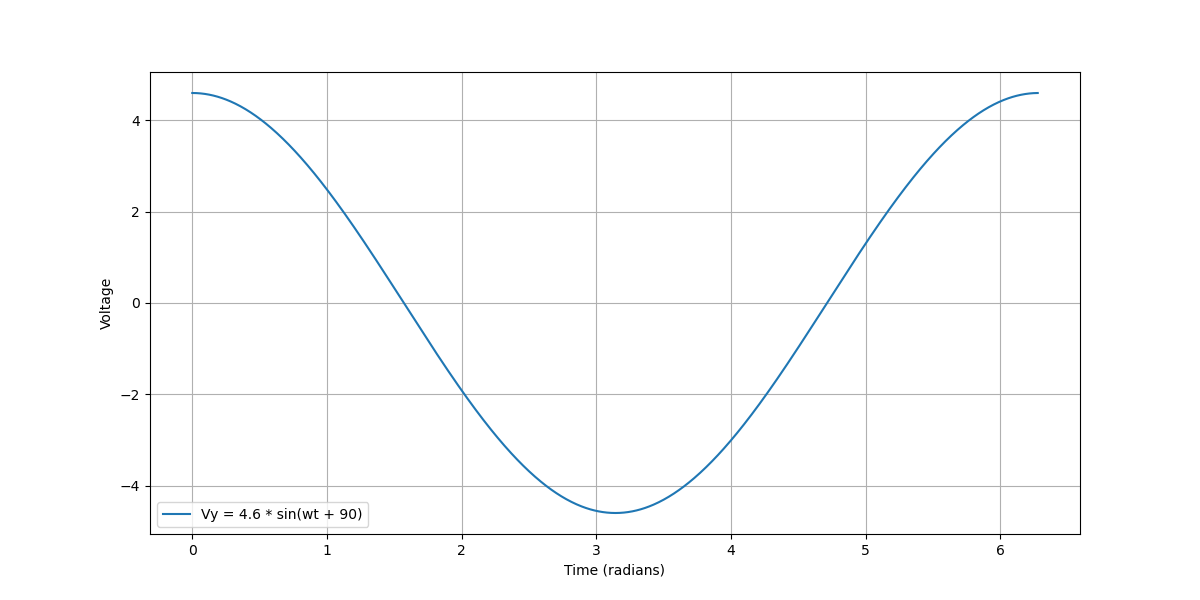
\includegraphics[width=1\linewidth]{2023/IN/61/figs/V_y.png} % Adjust the width as needed
        \caption{$plot of V_y$}
\end{figure}
\begin{figure}[h]
      \centering
       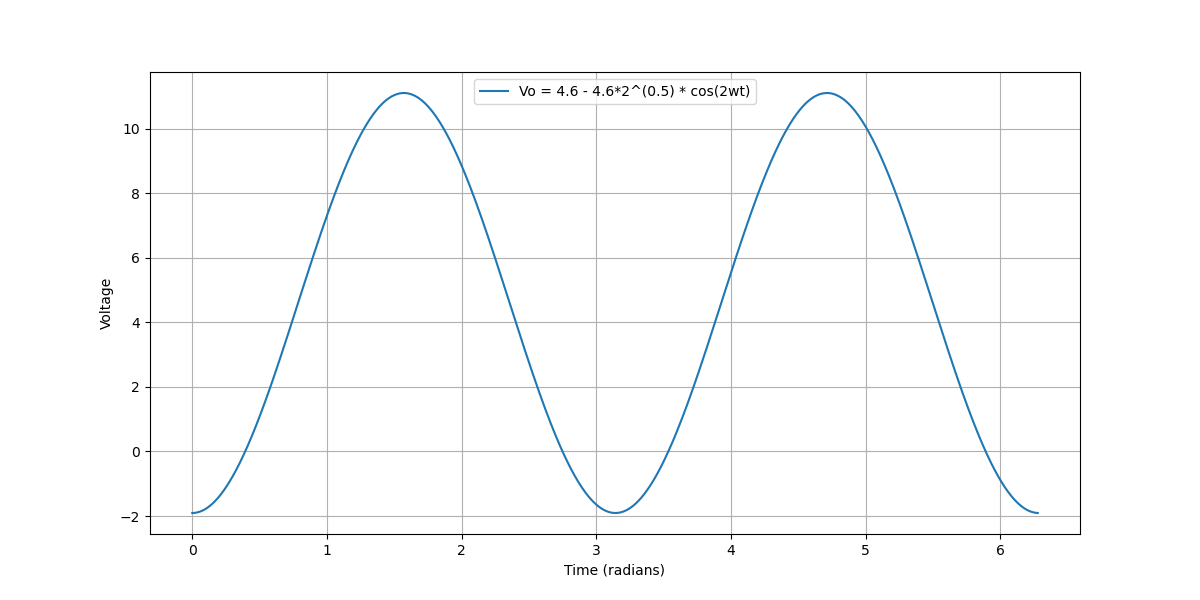
\includegraphics[width=1\linewidth]{2023/IN/61/figs/V_o.png} % Adjust the width as needed
        \caption{$plot of V_o$}
\end{figure}
%\end{document}
